\documentclass[11pt]{article}

% Packages
\usepackage[margin=2cm]{geometry}
\usepackage{amsmath} 
\usepackage{enumitem} 
\usepackage{amsfonts}
\usepackage{amsthm}
\usepackage{graphicx}
\usepackage{babel,blindtext}
\usepackage{float}
\usepackage{hyperref}

% Examples, definitions, theorems, etc
\theoremstyle{definition}
\newtheorem{ex}{Example}[section]
\newtheorem{defn}{Definition}[section]
\newtheorem{rmk}{Remark}[section]
\newtheorem{prop}{Proposition}[section]
\newtheorem{lem}{Lemma}[section]

\theoremstyle{theorem}
\newtheorem{thm}{Theorem}[section]

% Short-cuts
\newcommand{\R}[0]{\mathbb{R}}
\newcommand{\N}[0]{\mathbb{N}}

\newcommand{\prob}[1]{\mathbb{P}(#1)}
\newcommand{\expec}[1]{\mathbb{E}[#1]}
\newcommand{\comp}[1]{{#1}^{\texttt{C}}}
\newcommand{\borel}[0]{\mathcal{B}(\R)}
\newcommand{\pisys}[0]{\mathcal{I}}
\newcommand{\dsys}[0]{\mathcal{D}}

\begin{document}
\begin{center}
	\textbf{MATH 587: Numerical Analysis 1} \\
	\textbf{Task 1: Due 27 September 2021} \\
	\textbf{Shereen Elaidi (260727874)}
\end{center}
\textbf{0. The Lagrange Interpolation}
\newline
The Lagrange interpolating polynomial is expressed as a linear combination of the following basis polynomials: 
\begin{align*}
	\ell_j(x) := \prod_{i = 1, i\neq j}^N \frac{x-x_i}{x_j -x_i}.
\end{align*}
The weights in the linear combination of the \( \ell_j(x) \)'s correspond to the actual values of the function we are trying to interpolate, which we'll denote \( f(x_j) \). Therefore, the Lagrange interpolating polynomial \( p(x) \) is given by: 
\begin{align*}
	p(x) = \sum_{i=1}^N f(x_i) \ell_i(x).
\end{align*}
In this task we implement this interpolation in Python and test it on three functions:
\begin{align*}
u(x) = \sin(x),\ v(x) = \text{ Heaviside}(x), \text{ and } w(x) = \frac{1}{10x^2 + 1}.
\end{align*}
\textbf{1. Plots for Equidistant Spacing}
\begin{figure}[H]
\minipage{0.32\textwidth}
  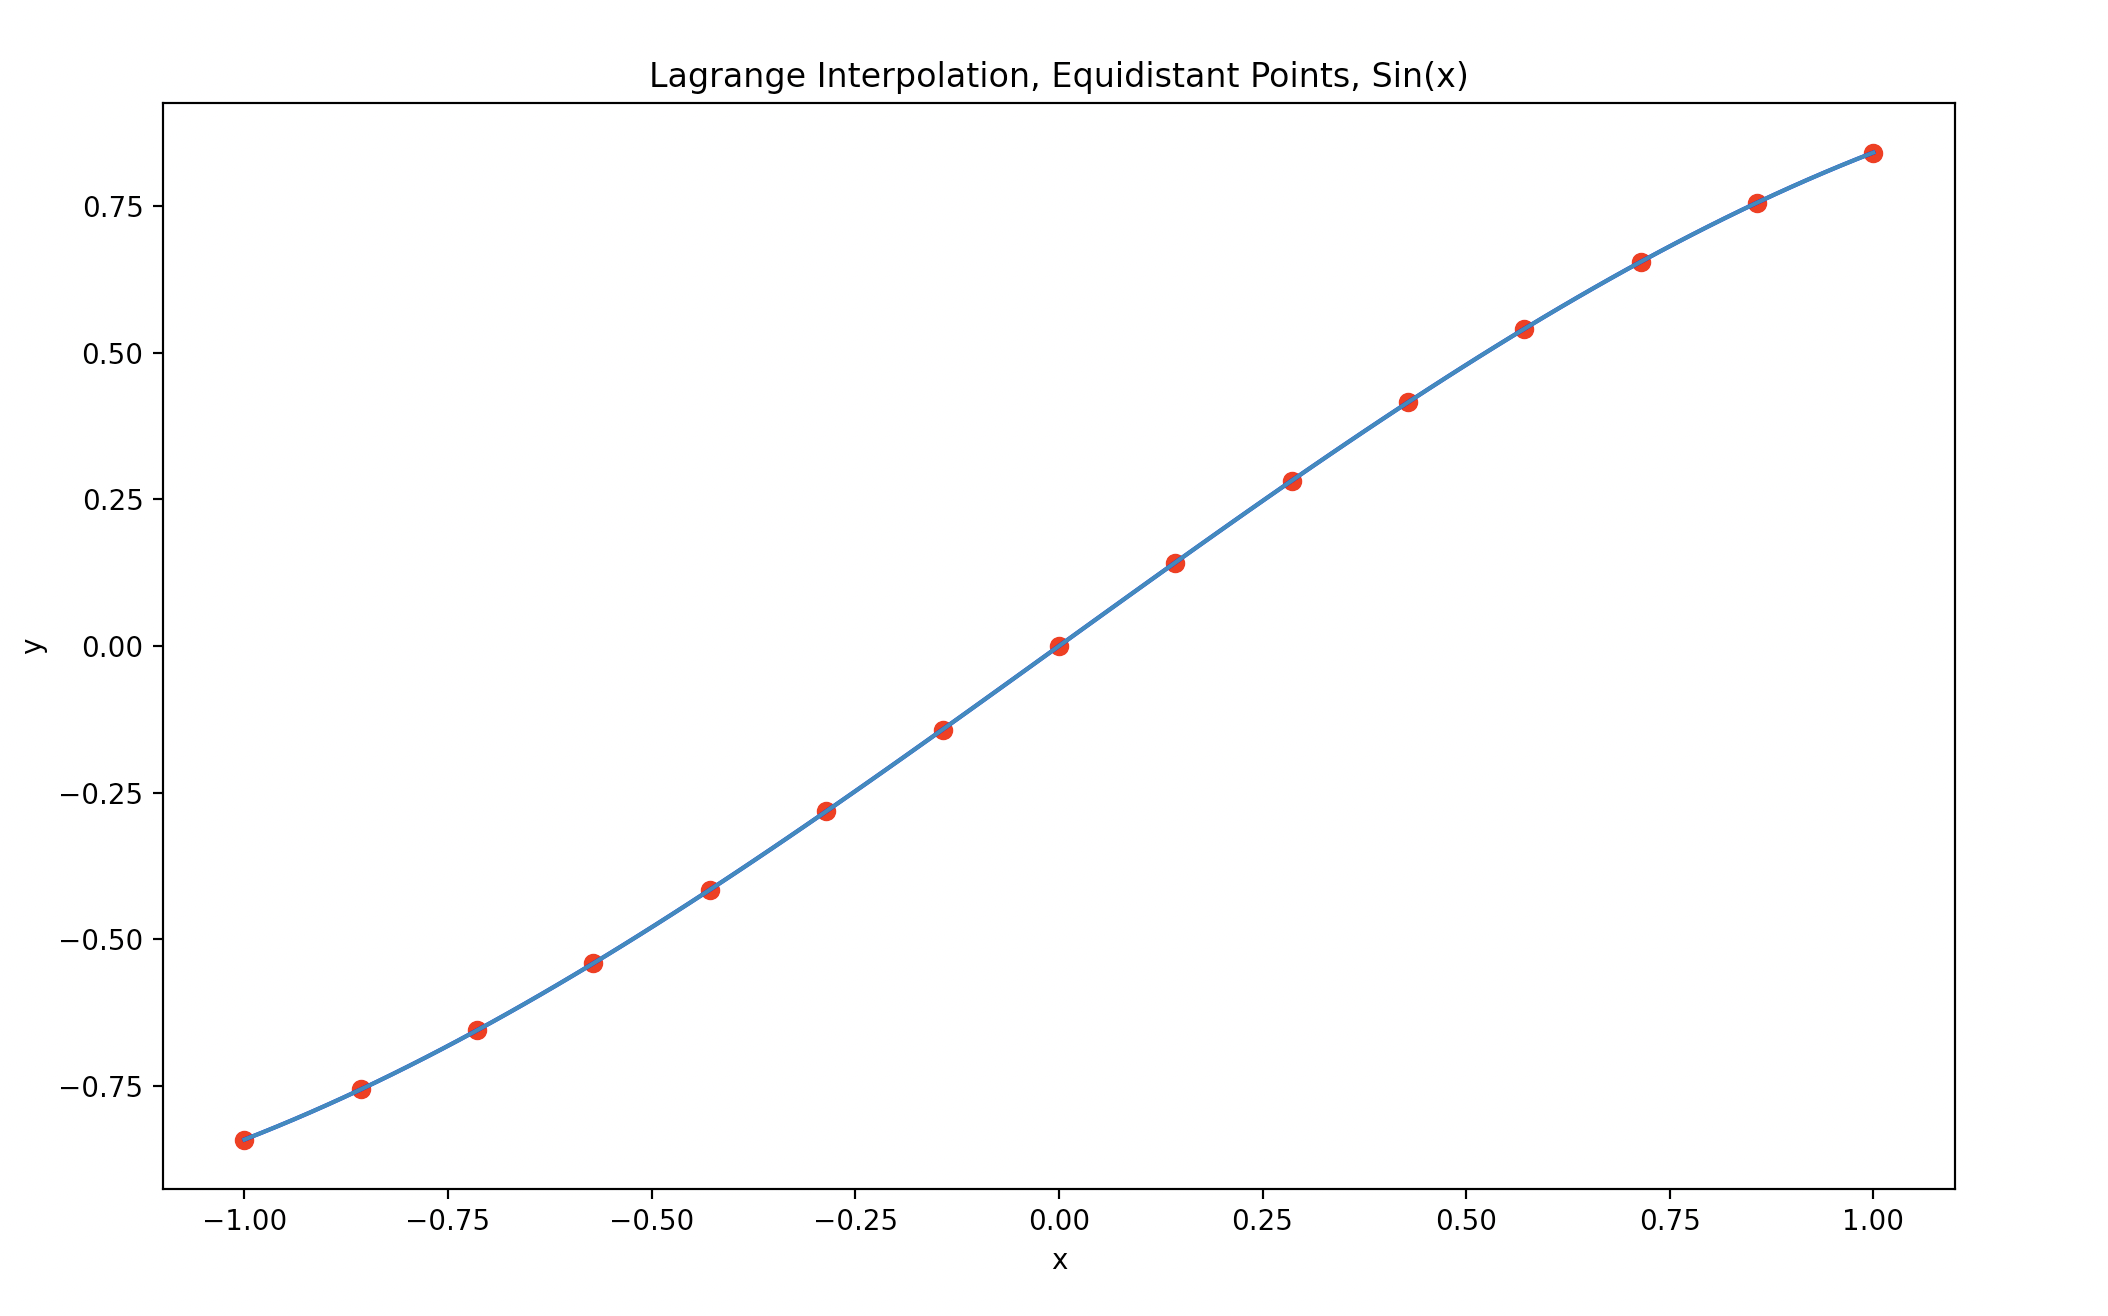
\includegraphics[width=\linewidth]{plots/1a.png}
  \caption{\( f(x) = \sin(x). \)}\label{fig:1a}
\endminipage\hfill
\minipage{0.32\textwidth}
  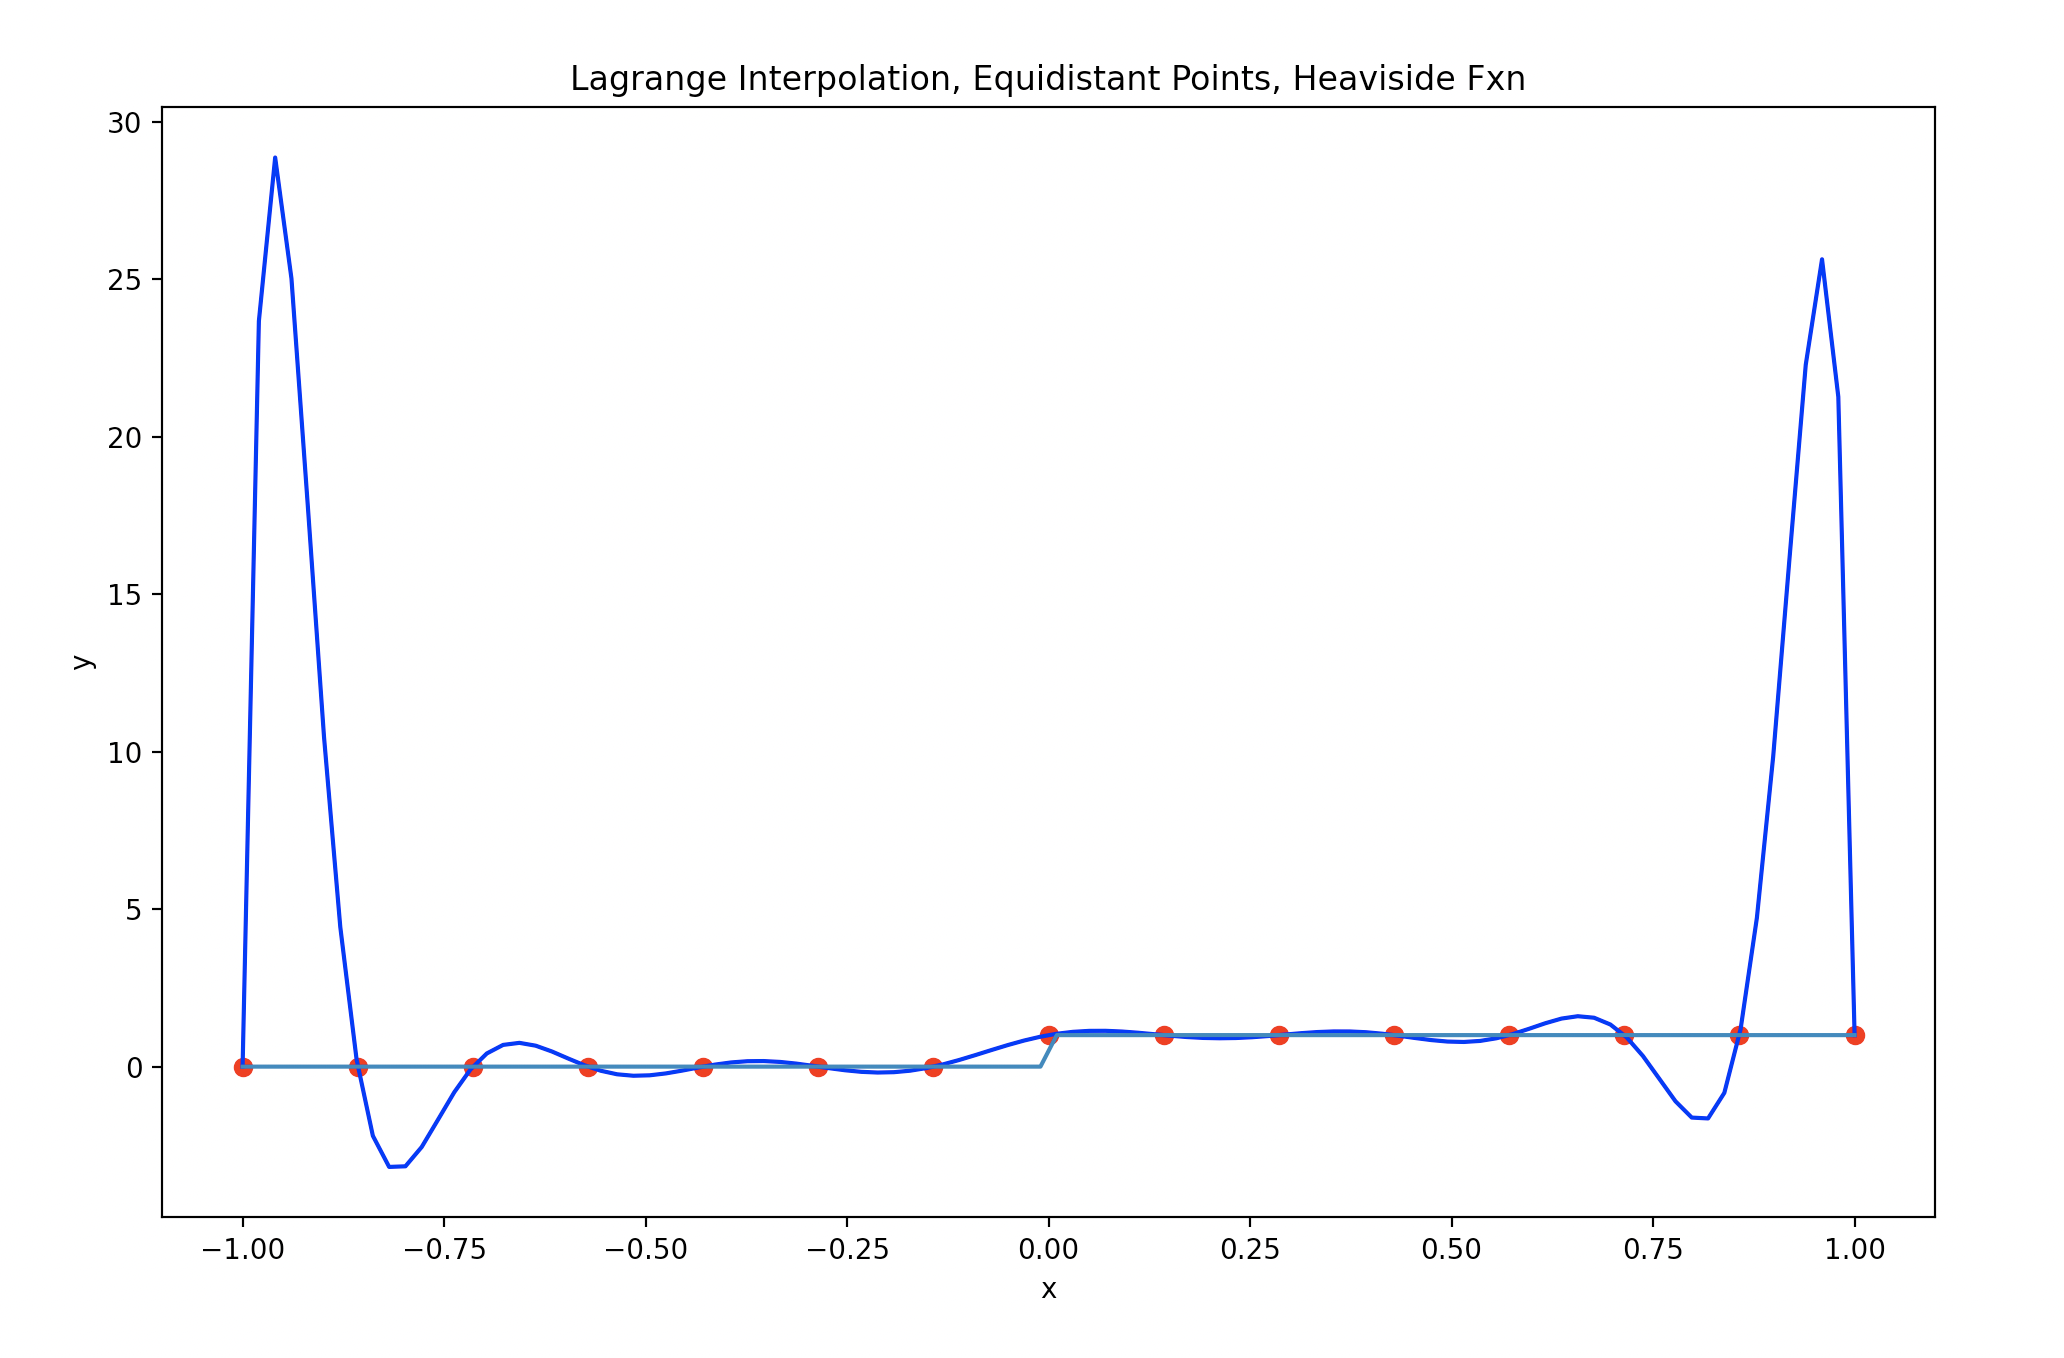
\includegraphics[width=\linewidth]{plots/1b.png}
  \caption{Heaviside function.}\label{fig:1b}
\endminipage\hfill
\minipage{0.32\textwidth}%
  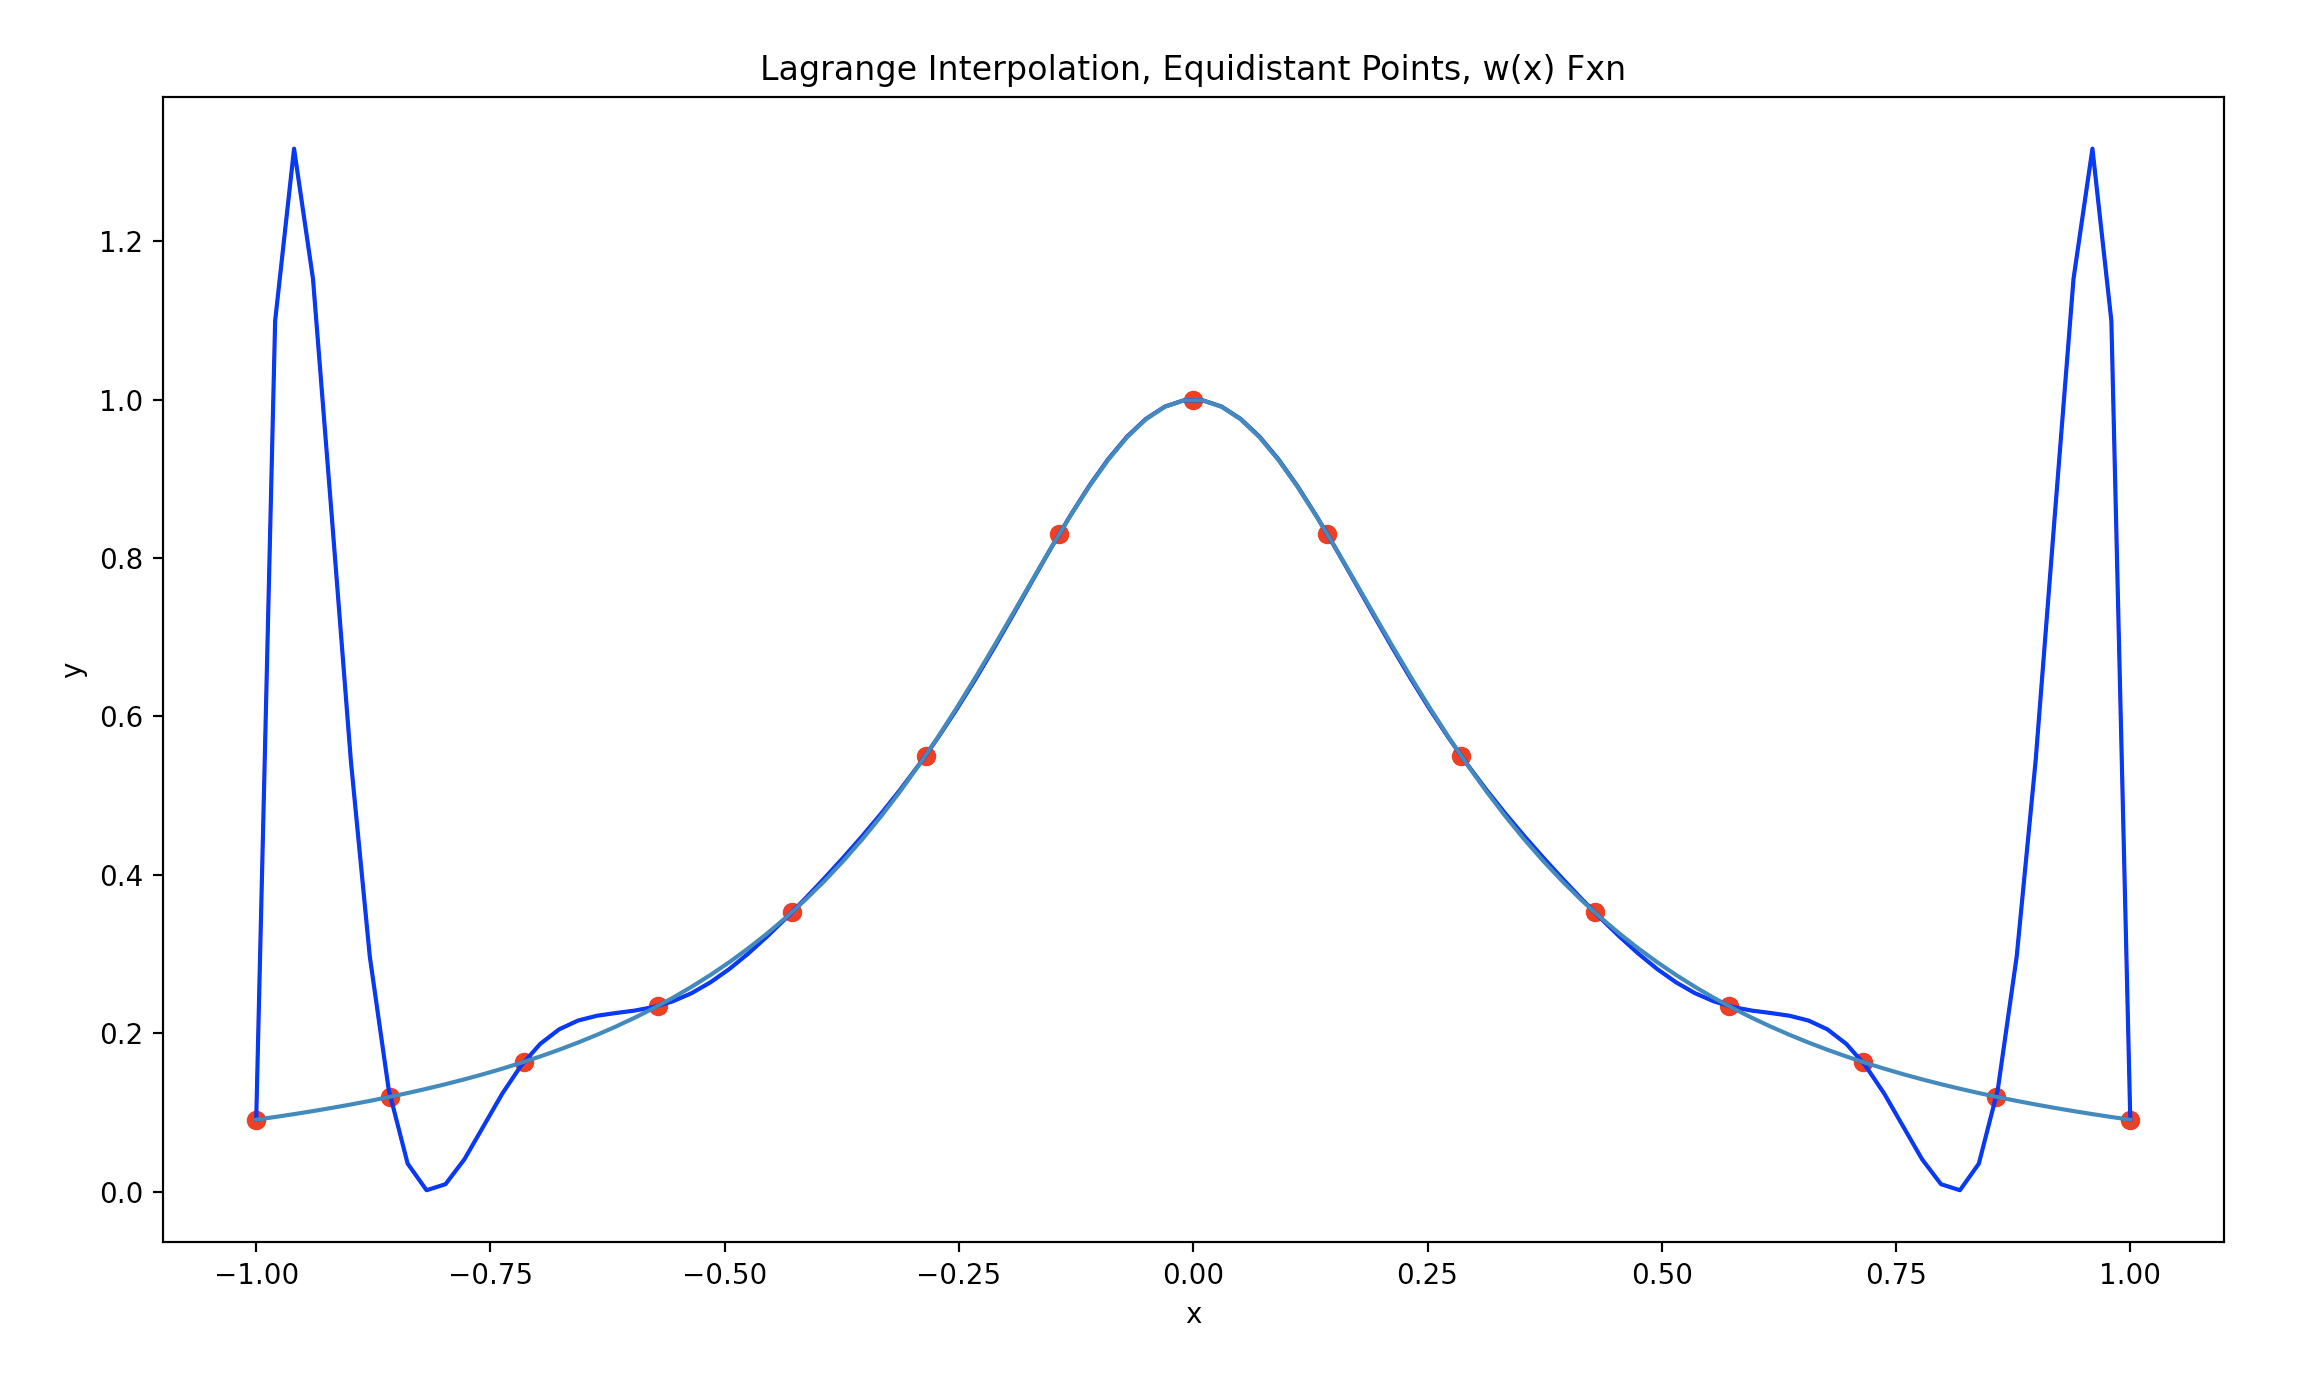
\includegraphics[width=\linewidth]{plots/1c.png}
  \caption{\(f(x) = \frac{1}{10x^2 +1}. \)}\label{fig:1c}
\endminipage
\end{figure}
The sharp blue colour corresponds to the plot of the interpolating polynomial. The other blue colour corresponds to the original function. We notice that in Fig. \ref{fig:1a}, the Lagrange fit is really good in \( [-1,1] \) compared to the fit in Fig. \ref{fig:1b} and Fig. \ref{fig:1c}, especially at near the endpoints of \( [-1,1] \). This behaviour seems to be irrelevant of the smoothness of the function we are trying to interpolate: the interpolation by the endpoints is very poor for both a discontinuous function (the Heaviside function) and a very smooth function (\( w(x) = \frac{1}{10x^2 +1} \)).

\textbf{2. Plots for Chebychev Spacing}
\begin{figure}[H]
\minipage{0.32\textwidth}
  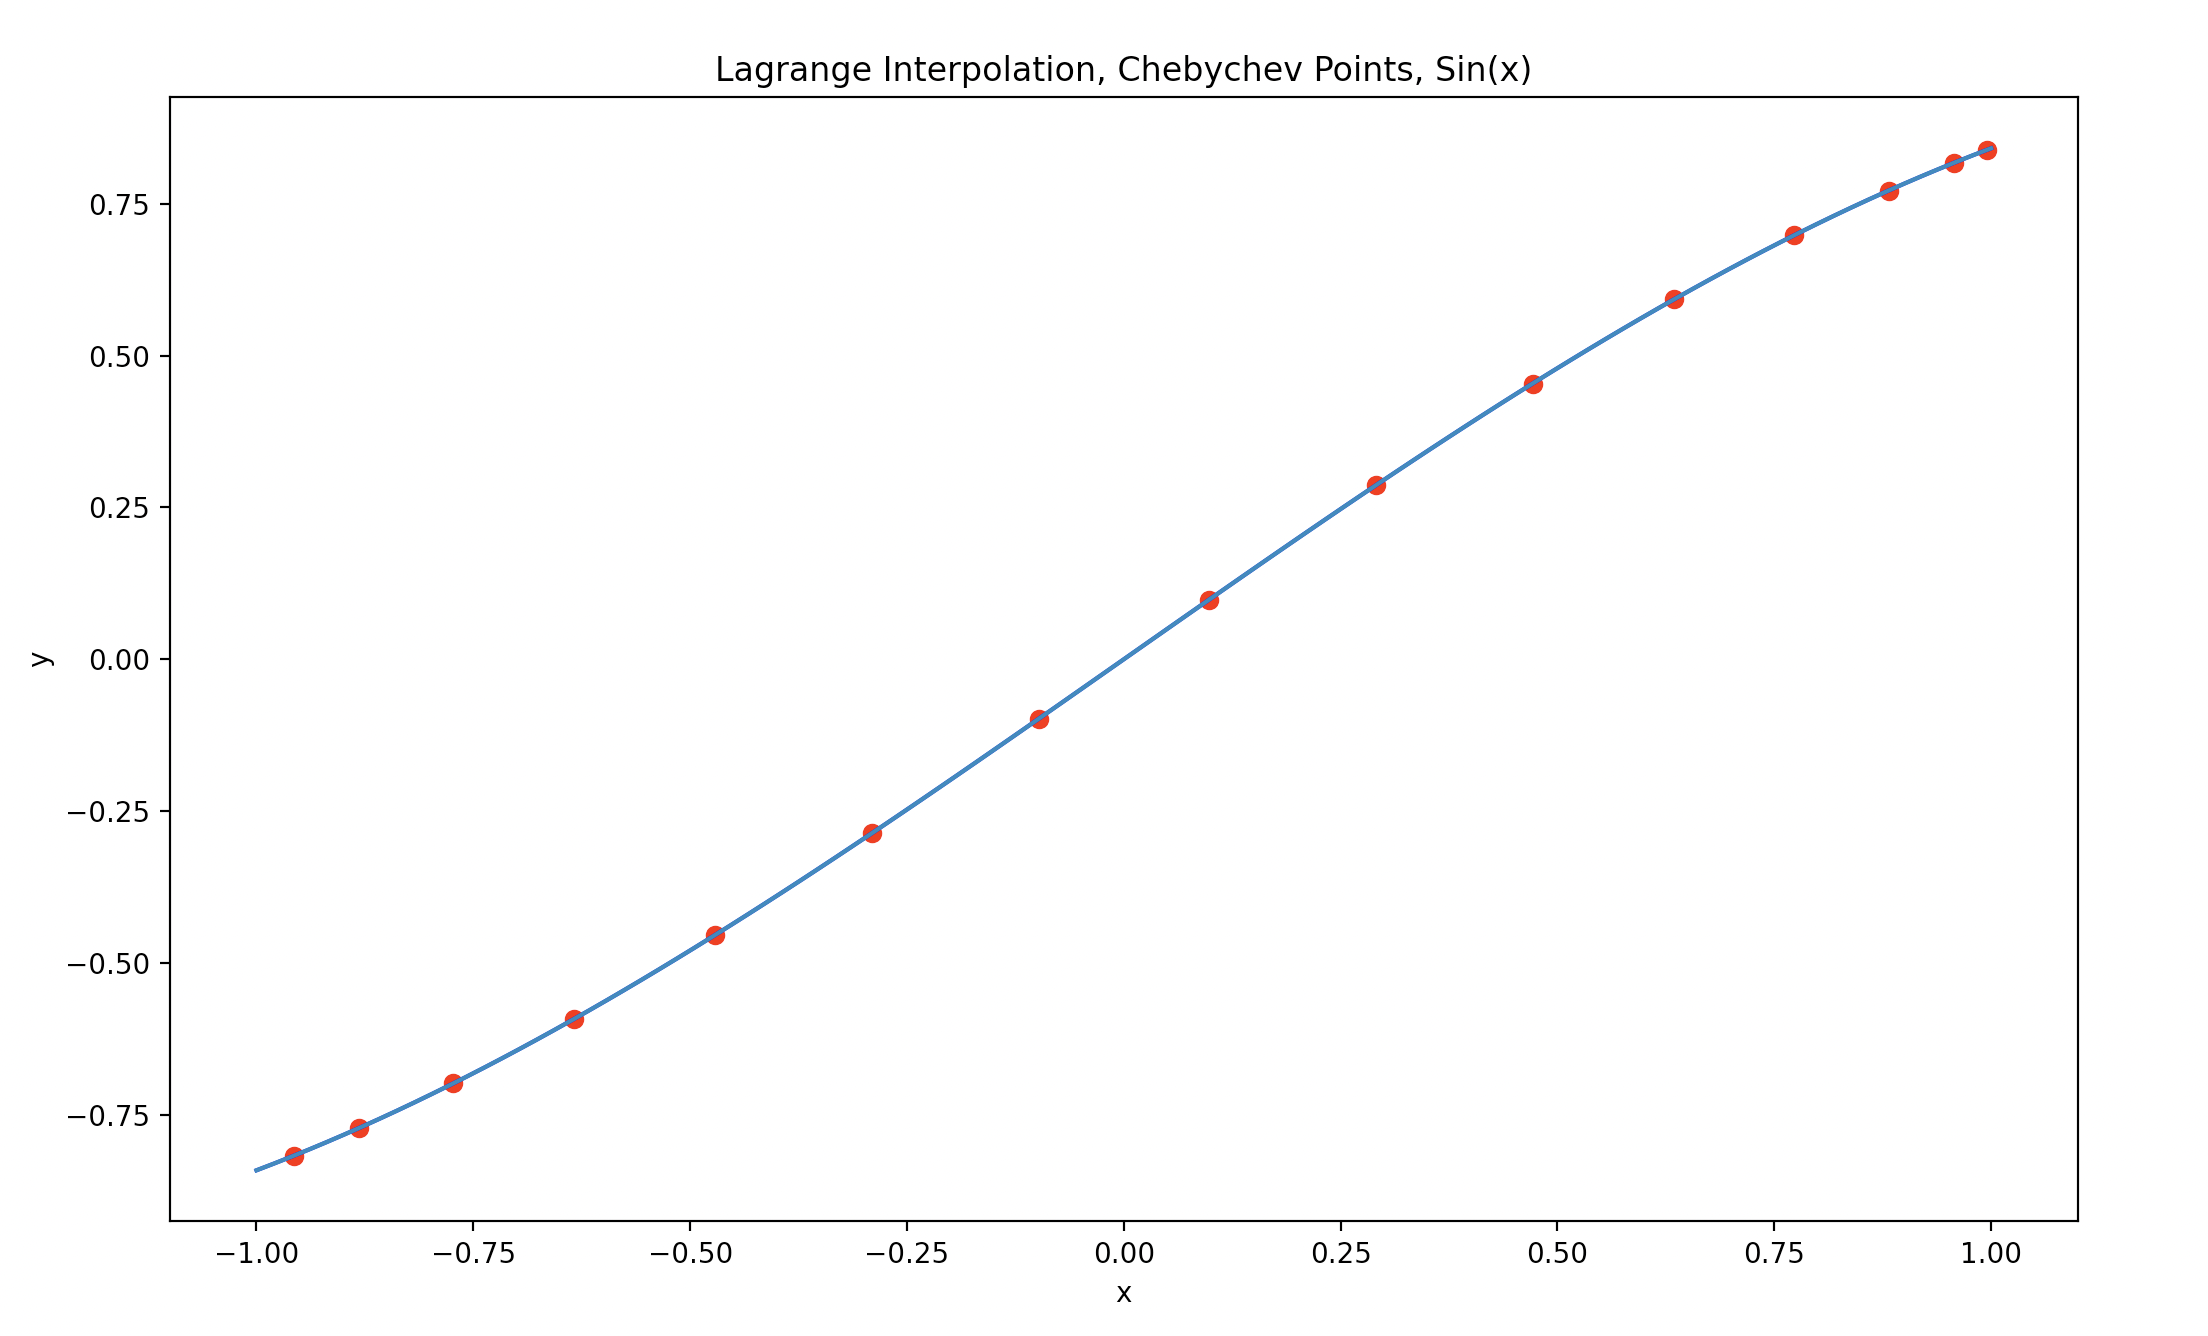
\includegraphics[width=\linewidth]{plots/2a.png}
  \caption{\( f(x) = \sin(x). \)}\label{fig:2a}
\endminipage\hfill
\minipage{0.32\textwidth}
  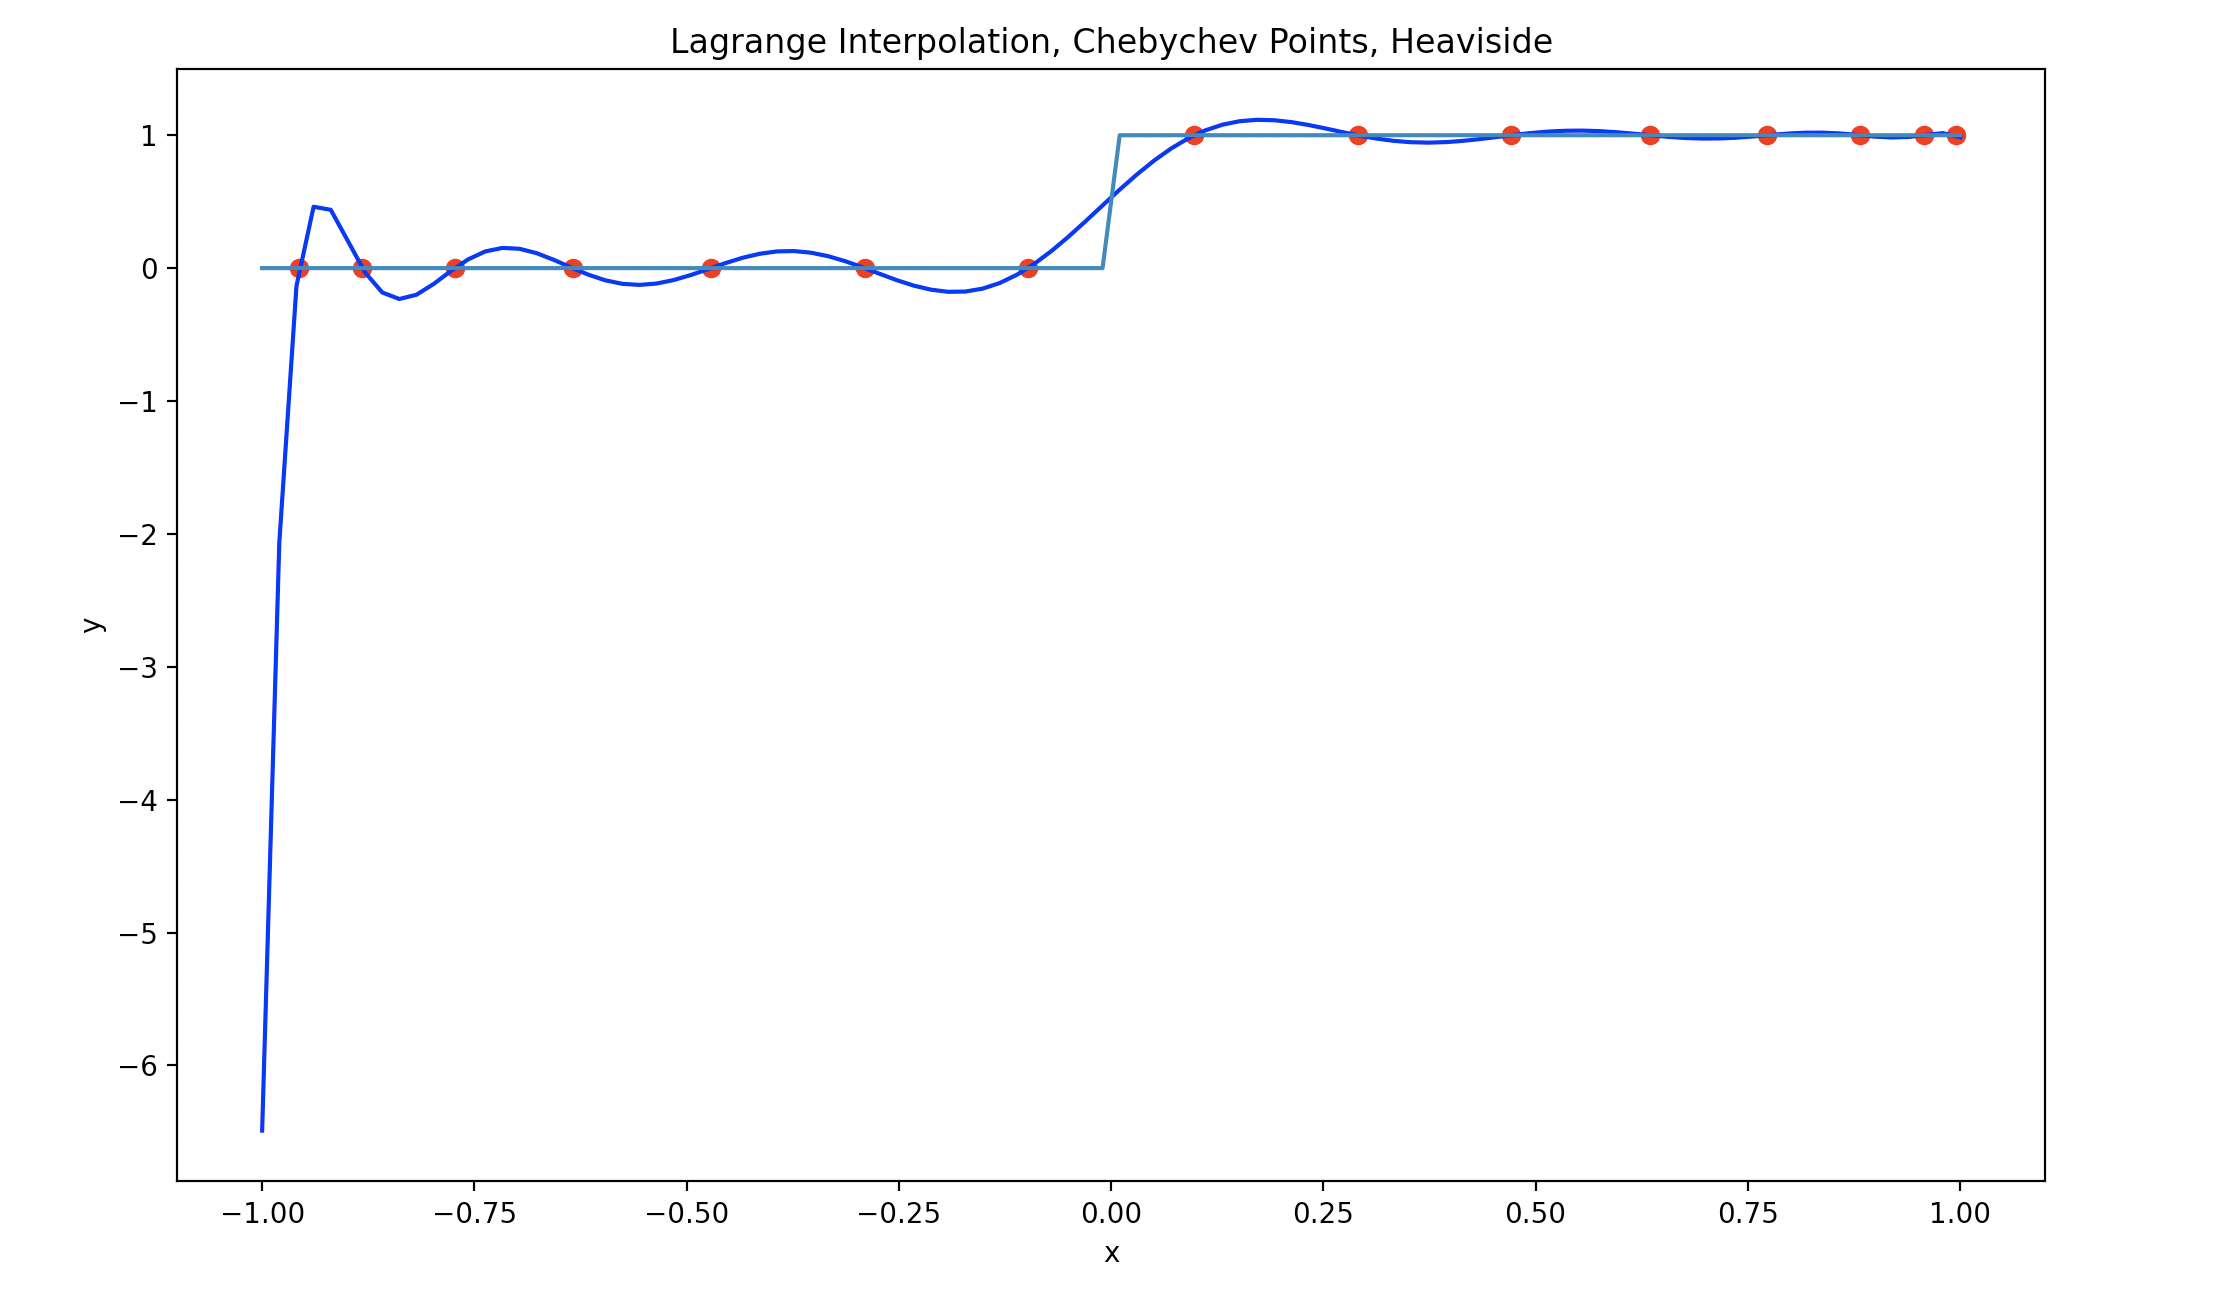
\includegraphics[width=\linewidth]{plots/2b.png}
  \caption{Heaviside function.}\label{fig:2b}
\endminipage\hfill
\minipage{0.32\textwidth}%
  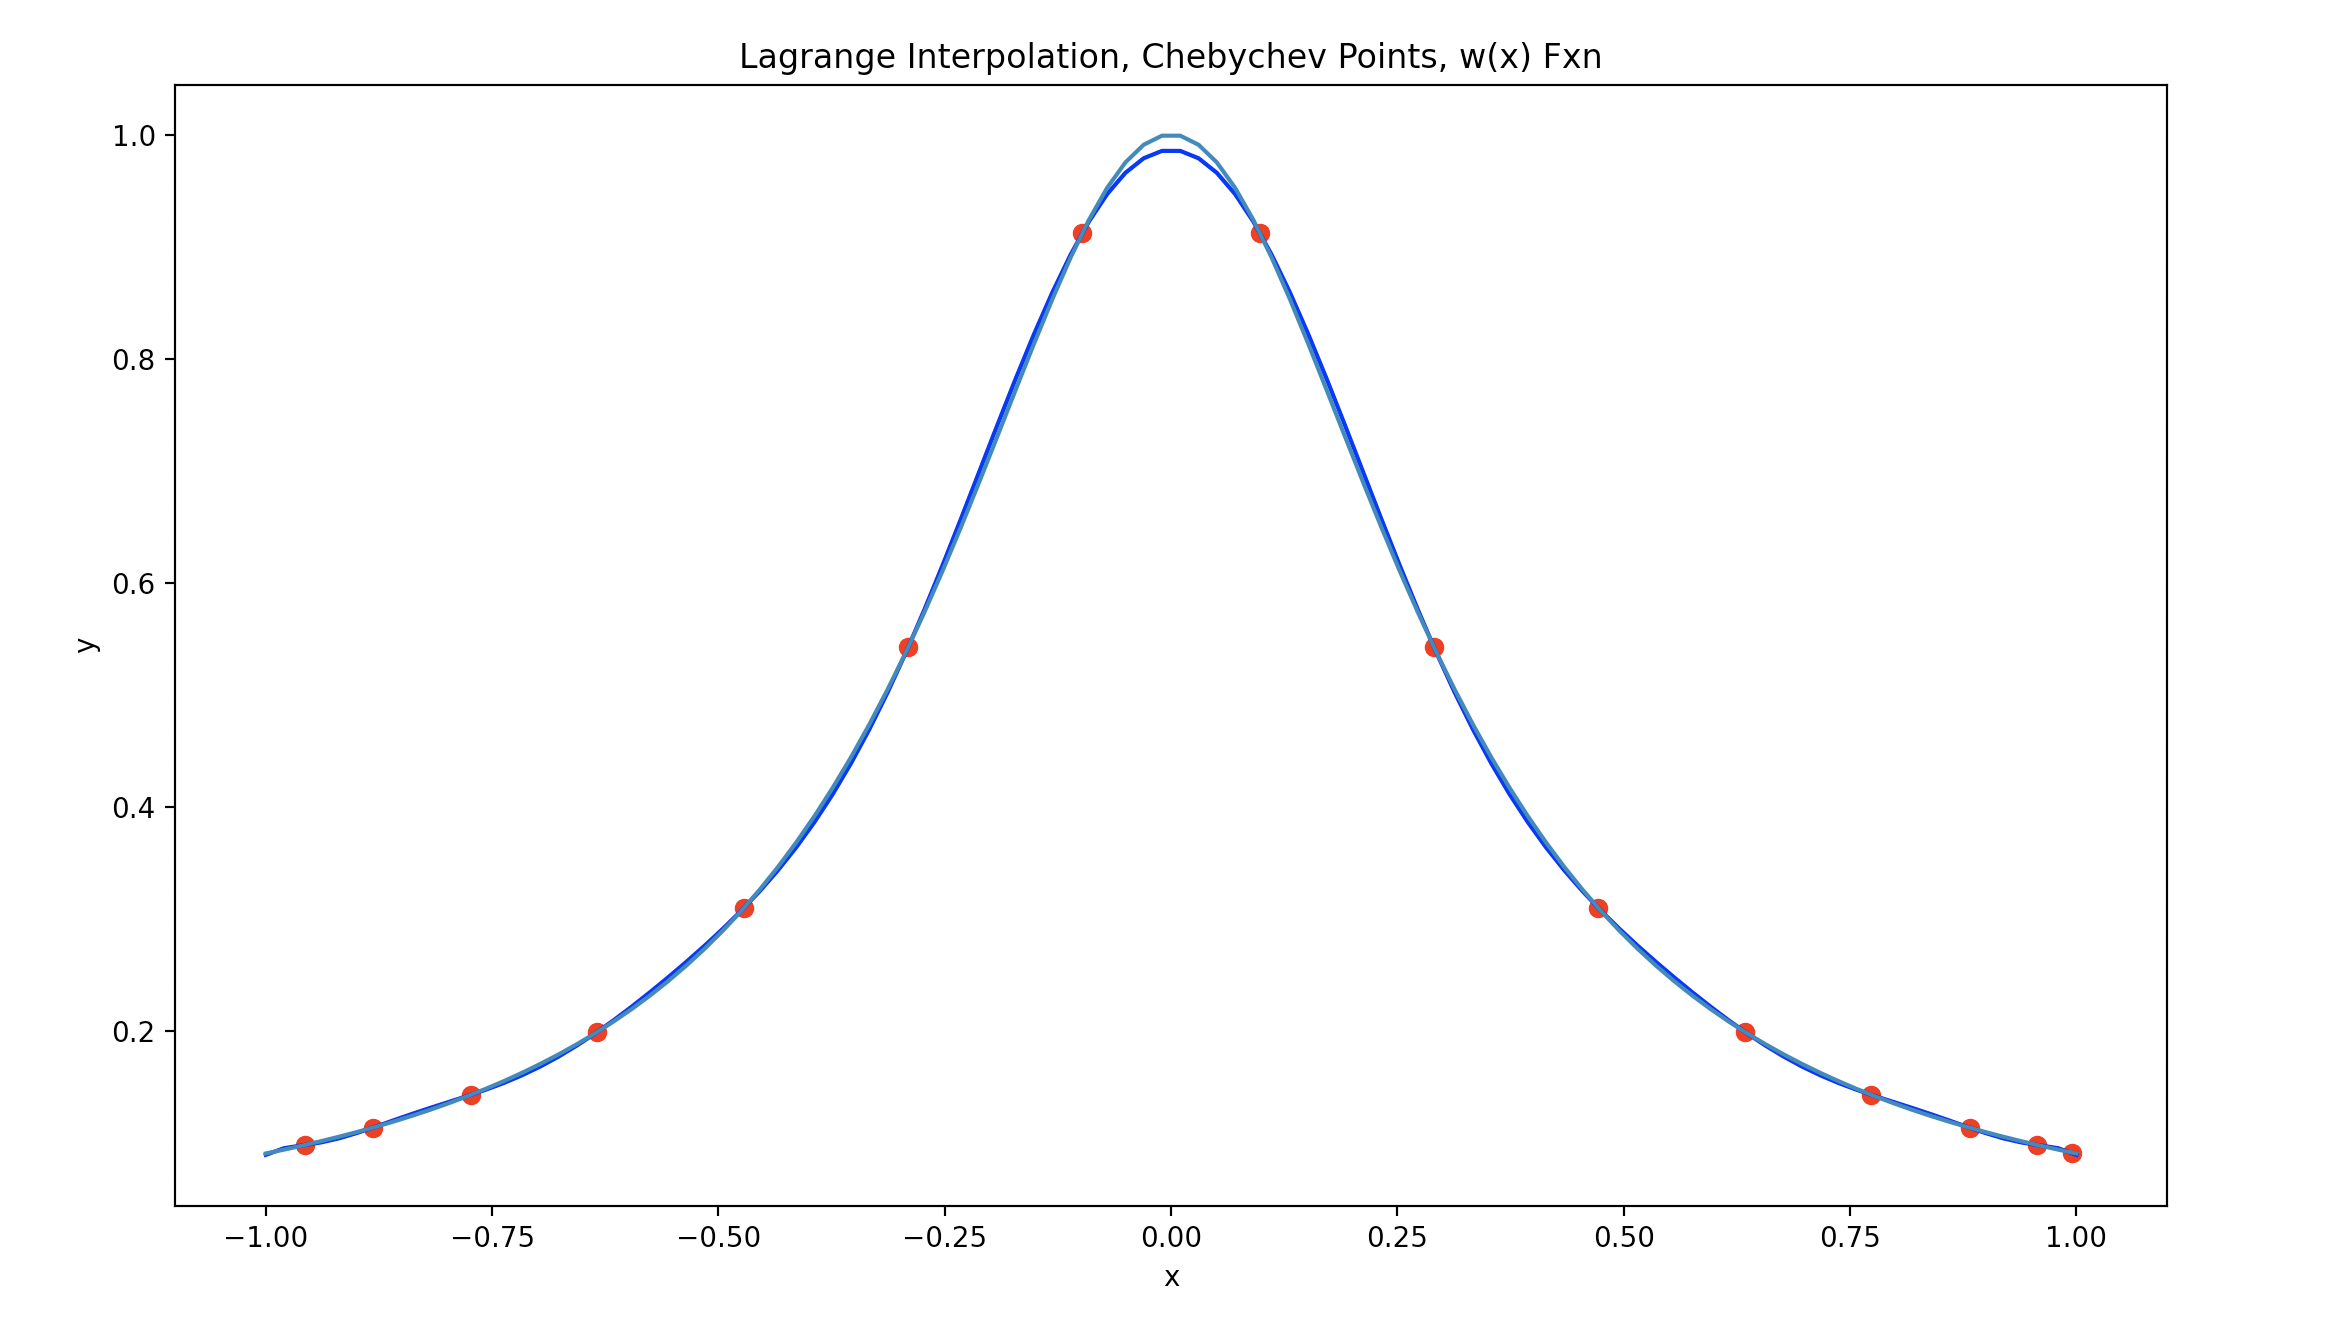
\includegraphics[width=\linewidth]{plots/2c.png}
  \caption{\(f(x) = \frac{1}{10x^2 +1}. \)}\label{fig:2c}
\endminipage
\end{figure}
For Chebychev points, we need to choose the roots of the 15th (since \( N = 15 \)) Chebychev polynomial. From lecture, we know those are the following points: 
\begin{align}
	\xi_j = \cos \left(  \frac{(2j + 1) \pi}{2N + 2} \right),\ j =0, ..., N.	
\end{align}
Otherwise, the code is exactly the same. We immediately see that the interpolation at the end points for the Heaviside function (Fig. \ref{fig:2b}) and \( w(x) \) (Fig. \ref{fig:2c}) performs much better than the equidistant point spacing in Fig. \ref{fig:1b} and Fig. \ref{fig:1c}. 

\textbf{3. Appendix}
\newline
The code for this assignment is in two files: the implementation of the Lagrange interpolation polynomial for a general case can be found in the file \texttt{lagrange.py} and the code to run our specific functions and specific point spacings can be found in the file \texttt{task1.py} (uploaded on myCourses). Just in case, both files are also on GitHub: \url{https://github.com/ShereenElaidi/math-578/tree/master/task-1}.

\end{document}